\documentclass{mc2015}

%%%%%%%%%%%%%%%%%%%%%%%%%%%%%%%%%%%%%%%%%%%%%%%%%%%%%%%%%%%%%%%%%%%%%
\usepackage[T1]{fontenc}         % Use T1 encoding instead of OT1
\usepackage[utf8]{inputenc}      % Use UTF8 input encoding
\usepackage{microtype}           % Improve typography
\usepackage{booktabs}            % Publication quality tables
\usepackage{amsmath}
\usepackage{graphicx}
\usepackage{caption}
\usepackage{subcaption}
\usepackage{float}
\usepackage[exponent-product=\cdot]{siunitx}
\usepackage[colorlinks,breaklinks]{hyperref}
\hypersetup{linkcolor=black, citecolor=black, urlcolor=black}

\def\equationautorefname{Eq.}
\def\figureautorefname{Fig.}

%%%%%%%%%% MC JOURNAL NOTES %%%%%%%%%%%%%%%%%%%%%%%%%%%%%%%%%%%%%%%%%
%
% References can be typeset properly using the provided \textsc{Bib}\TeX style file. See examples of a journal~\cite{journal}, conference proceedings~\cite{proceedings}, book~\cite{book}, and miscellaneous~\cite{misc}.
%
%References to websites are discouraged, but acceptable if absolutely necessary.  It is the author?s responsibility to check links in the pdf file.
%Final PDF file size should be no more than 4 MB.  Recommended paper length is 10-12 pages.
%
% Subsection Title: First Character of Each Non-trivial Word is Uppercase
%Equations (Equation \ref{eqn:sample}) should be centered and sequentially numbered to the flush right of the formula.
% Sub-subsection level and lower: only first character uppercase
%
%\begin{equation}
%  1+1=2 \label{eqn:sample}
%\end{equation}
% The continuation of a paragraph after an equation is not indented
%
%Figures and tables should appear as closely as possible to where they are first cited, e.g. Fig. \ref{fig:sample}, in the text.  Figures are numbered in Arabic numerals, with the caption centered below the figure, in boldface. 
%
%\begin{figure}[H]
%  \centering
%  \includegraphics[width=3in]{figure.png}
%  \caption{Sample Figure. Color is permitted, but must be readable if printed.}
%  \label{fig:sample}
%\end{figure}
%
% When importing figures or any graphical image please verify two things:
% 1. Any number, text or symbol is no smaller than 10-point after reduction to the actual window in your paper;
% 2. That it can be translated into PDF.
%
% Tables, like Table \ref{tab:sample}, are numbered in Roman numerals, with the caption centered above the table, in \textbf{boldface}.  
% Double-space before and after the table.
%
%\begin{table}
%  \centering
%  \caption{Sample table: accuracy of nodal and characteristic methods}
%  \begin{tabular}{lcccc}
%    \toprule
%    Mesh & 8 x 8 & 16 x 16 & 32 x 32 & 64 x 64 \\
%    \midrule
%    Nodal & \num{1.000e-1} & \num{2.500e-2} & \num{6.250e-3} & \num%{1.563e-3} \\
%    Characteristic & \num{1.000e-1} & \num{2.500e-2} & \num{6.250e-3} & \num{1.563e-3} \\
%    \bottomrule
%  \end{tabular}
%  \label{tab:sample}
%\end{table}


%%%%%%%%%%%%%%%%%%%%%%%%%%%%%%%%%%%%%%%%%%%%%%%%%%%%%%%%%%%%%%%%%%%%%
% Insert authors' names and short version of title in lines below

\authorHead{Shaun Marshall, Blake Currier, Andrew D Hodgdon}
\shortTitle{Proton Gain in Faraday Cup}


%%%%%%%%%%%%%%%%%%%%%%%%%%%%%%%%%%%%%%%%%%%%%%%%%%%%%%%%%%%%%%%%%%%%%
\begin{document}

\title{Proton-Induced Gain in a Portable Faraday Cup}

\author{Shaun Marshall}
\author{Blake Currier}
\affil{
Department of Physics \\
Worcester Polytechnic Institute \\
100 Institute Rd, Worcester, MA 01609
}

\author{Andrew D Hodgdon, CHP}
\affil{
Radsim, LLC \\
584 Grove St, Newton, MA 02462 \\
adhodgdon@radsim.org
}

\maketitle

\begin{abstract}
A Faraday Cup (FC) is being designed to calibrate therapy-range proton accelerators, i.e., 50 to 250 MeV. The FC must be accurate to 1\% as well as portable, hence vacuum-less and low mass. The FC is a copper cylinder coated with kapton insulation and silver ground. The Monte Carlo method (MCNP6 and Geant4) was used to simulate the radiation cascade and predict gain versus height (H), diameter (D) and insulator thickness (K). H and D were mostly functions of proton range. Increasing either increases mass, reducing either increases proton leakage, hence decreases accuracy. Kapton functions to capture backscattered electrons, the function of the fields in a standard FC. Greater K increases capture but increases secondary electron in-leakage. Determining optimal K was made difficult by the lack of low energy proton, electron cross-sections. A secondary electron model was programmed with the SDEF command for the MCNP model based on recently published cross-section approximations. This secondary electron source method was benchmarked against a series of experimental measurements (by others) of protons on copper and on water. Three FCs were built, each with different values of K. They are currently being tested. 

\emph{Key Words}: Monte Carlo, Geant, MCNP, Faraday Cup
\end{abstract}


%%%%%%%%%%%%%%%%%%%%%%%%%%%%%%%%%%%%%%%%%%%%%%%%%%%%%%%%%%%%%%%%%%%%%
\section{Introduction}

In modern day radiation therapy, protons have become one increasingly popular method of treating cancer near critical structures, with many dosimetric advantages of charged particle interactions (References). A novel portable vacuumless Faraday Cup measuring device was designed to calibrate proton therapy facilities, in energies ranging from 50 to 250 MeV. The detector is constructed of a copper cylinder, coated with kapton insulation and grounded with silver (Reference). Monte Carlo computational simulations in MCNP6 (Reference) and GEANT4 (Referenced) were performed to evaluate radiation cascade effects and predict signal versus height, diameter and insulator thickness characteristics.

Preliminary results indicated that increasing the mass of the Faraday Cup’s conductor reduced proton leakage but increased the system accuracy. While a greater kapton thickness increases the capture of primary and secondary electrons, it also increases secondary electron leakage. Additionally, determining the optimal kapton thickness has been made difficult by the lack of low energy proton and electron cross-sections in current Monte Carlo based simulation programs (Reference). A comprehensive secondary electron evaluation of the kapton was performed and benchmarked against a series of experimental measurements by Borovsky et al.1 and J. Gordon et al (Reference).

In conjunction with the computational calculations, three (3) prototype Faraday Cup measuring devices were constructed by Pyramid Technical Consultants, Inc. (Waltham, Ma), each having a different thickness of kapton. The units were tested in Germany to determine accuracy of the new design. 


%%%%%%%%%%%%%%%%%%%%%%%%%%%%%%%%%%%%%%%%%%%%%%%%%%%%%%%%%%%%%%%%%%%%%
\section{Experimental Background}


\subsection{Heidelberg Institute of Technology}

Table \ref{tab:HIT_data}

\begin{table}
  \centering
  \caption{Measured Gain from HIT Beam Stops}
  \begin{tabular}{lccccc}
    \toprule
    Energy (MeV) & S59 & S100 & S200 \\
    \midrule
    70.03  & \num{0.9750} & \num{0.9385} & \num{0.9350} \\
    100.46 & \num{0.9850} & \num{0.9500} & \num{0.9475} \\
    130.52 & \num{0.9925} & \num{0.9580} & \num{0.9525} \\
    160.09 & \num{1.0000} & \num{0.9635} & \num{0.9590} \\
    190.48 & \num{1.0075} & \num{0.9715} & \num{0.9650} \\
    221.06 & \num{1.0125} & \num{0.9800} & \num{0.9770} \\
    \bottomrule
  \end{tabular}
  \label{tab:HIT_data}
\end{table}

\subsection{GO14}


\subsection{BO88}


\section{Simulation Results}


\subsection{MCNP6}

MCNP version 6.1 with standard cross-section libraries was used to simulate gain. The material geometry is shown in Fig. \ref{fig:model_geometry} The height of the cylinder is fixed at 10 cm. The diameter is varied from 2 to 10 cm and the Kapton thickness is varied from 25 to 75 microns. The materials are standard copper, Kapton, silver and air at STP. The source is a 2 cm diameter proton beam at 250 MeV. This is the maximum expected energy. A suitable diameter for this energy will be suitable for lower energies. Physics was turned on for seven particles: neutrons, photons, electrons, protons, deuterons, tritons and alphas.

\begin{figure}[H]
  \centering
  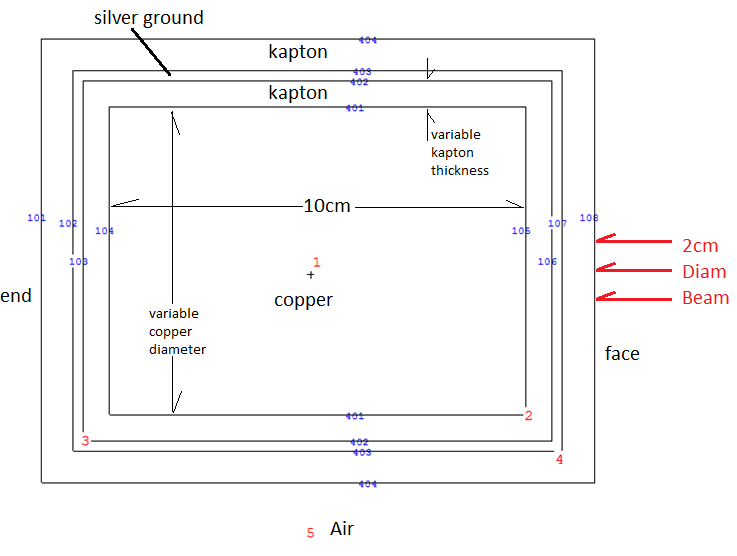
\includegraphics[width=5in]{fig_geometry.png}
  \caption{Geometry from side of horizontal copper cylinder}
  \label{fig:model_geometry}
\end{figure}

Gain was modeled simplistically by tallies of two charged particles (protons and electrons) crossing three surfaces (face, side and end). Gain is expressed in terms of elemental charge deposited in copper per beam proton, shown in eq. \ref{eqn:gain_definition}.

\begin{equation}
Gain = \frac{\sum Q_{particle\rightarrow Cu} - \sum Q_{particle\leftarrow Cu}}{\sum Q_{P+\ beam}}
\label{eqn:gain_definition}
\end{equation}

MCNP6 distinguishes between two types of secondary electrons, those that are created by proton collisions, i.e., SE$_h$, (MCNP cannot track such electrons) and those that are generated by other particles (notably photons that are themselves secondary), i.e., SE$_{!h}$. It was assumed that for the selection of a good copper diameter the SE$_h$ are not important. This assumption was not tested.

It is assumed that protons and electrons are the only contributors to gain. This was tested (for SE$_{!h}$ only) and found to be true within a factor of 2E-4.

It was also assumed that the detailed behavior of SE$_{!h}$ electrons in Kapton (i.e., capture causing mirror charge in copper) has little effect on the choice of copper diameter. This means that the location and energy of electrons captured in the kapton do not have to be tallied to get a good answer for the copper diameter; this assumption was not tested.

The detector is to be a beam proton counter. The perfect detector will yield a gain of unity, i.e., 1 exactly, seen in eq. \ref{eqn:error_definition}

\begin{equation}
Error = (Gain-1)\cdot100\%
\label{eqn:error_definition}
\end{equation}

\subsection{Geant4}

Geant4 is an object-oriented C++ toolkit for developing applications which simulate the passage of particles through matter. Libraries of cross-section tables, elemental/molecular properties, and pre-defined stochastic physics processes allow for rapid, intuitive invocation of necessary system setup commands. Once initialized, \lq\lq Manager" modules cooperate to organize and accumulate dynamic information which is organized in the following chronology:

\begin{enumerate}
\item The \textbf{DetectorConstruction} class is called to verify, store and lock the predefined geometry.
\item The \textbf{G4UIManager} initializes upon successful compilation and execution of the \emph{main()} routine.  If a visualizer is selected, \textbf{G4VisManager} is also invoked.
\item The user issues the command to execute a macro file of \emph{runs}; each run is characterized by the defined beam particle type, the beam energy, and the number of \emph{events}, or number of such isolated simulations.  If multithreading is available, \textbf{G4RunManager} allocates the events to the available worker threads on a rolling basis.
\item For each event, the simulation of the \emph{primary} (beam) particle proceeds, constructing a new \emph{track}, or well-defined trajectory for every particle not at rest.
\item The behavior of every track is determined dynamically, with each \emph{step}, or stochastically occuring physical process (collisions, absorbtions, etc) of the particle in some medium.
\end{enumerate}

\subsubsection{UserAction methods}

A useful feature of Geant4 is the ability to create user-defined actions (methods) throughout each module, which allows for a very fine-tuned analysis throughout the entire simulation.  The following summarizes the custom details and methods for this application

\begin{itemize}
\item \textbf{DetectorConstruction.cc:} A copper cylinder of radius 3 cm and height 10 cm is covered in Kapton film of varying thickenesses: 59 $\mu$m, 100 $\mu$m and 200 $\mu$m.  The film thickness is iterated by a function which is called before the command macro is examined.  The top face of the copper lies in the $z=0$ plane, with the beam approach the system from beneath.
\item \textbf{SteppingAction.cc:} [For every step,] immediately checks if the step is the finale of a track.  If so, the particle's vertex (original position) and destination volume and coordinates are found, and a charge signal calculation occurs.  Entering/Leaving the copper gives a net signal of $\pm q$ where $q$ is the charge of the particle.  Entering/Leaving Kapton gives a relative proportionality of

\begin{equation}
s_{q\rightleftharpoons KA} = \pm q\times\max\left[r_{\%}, z_{\%}\right], \label{eqn:s_KA}
\end{equation}

where $r_{\%}$ is the percent distance away from the copper radially and $z_{\%}$ is the percent distance away laterally.  The signals are grouped and saved by a unique eventID number.
\item \textbf{EventAction.cc:} At the end of each event, the signals are tallied, grouped, and saved by a unique runID number.
\item \textbf{RunAction.cc:} At the end of each run, the average and standard deviation of the signals are acquired.
\end{itemize}

\subsubsection{Experimental parameters}

Table \ref{tab:geant4setup} summarizes the detector geometry of each run.  The order of logical volume layers starting from the innermost are 1) the copper cylinder, 2) the Kapton1 film, 3) the silver paint layer, and 4) the Kapton2 film.  Constructing cylindrical \lq\lq layers" is as straightforward as defining a cylinder within another's logical volume.  Data were acquired as a function of impinging proton energy using the 50-250 MeV range as used in the HIT experiment.  The Kapton1 thickness optimization was applied to this model both with and without the silver and secondary Kapton (\emph{+Ag/KA}).

\begin{table}
  \centering
  \caption{Geant4 Simulation Cylindrical Construction}
  \begin{tabular}{ccc}
    \toprule
    Volume  & Radius (mm) & Height (mm) \\
    \midrule
    Copper  & \num{30} & \num{100} \\
    \toprule\toprule
            & Model    & Thickness ($\mu$m) \\
    \midrule
    Kapton1 & S59      & \num{59}  \\
            & S100     & \num{100} \\
            & S200     & \num{200} \\
    Silver  & +Ag/KA   & \num{12}  \\
    Kapton2 & +Ag/KA   & \num{62}  \\
    \bottomrule
  \end{tabular}
  \label{tab:geant4setup}
\end{table}


%%%%%%%%%%%%%%%%%%%%%%%%%%%%%%%%%%%%%%%%%%%%%%%%%%%%%%%%%%%%%%%%%%%%%
\section{Results}

(LATER: intro info here)

\subsection{MCNP6 Simulation}

Fig.~\ref{fig:error_diameter} shows the variation of error with copper diameter and method. Two methods are compared, SRIM (reference) and MCNP6. A diameter of 6cm seems reasonable.

\begin{figure}[H]
  \centering
  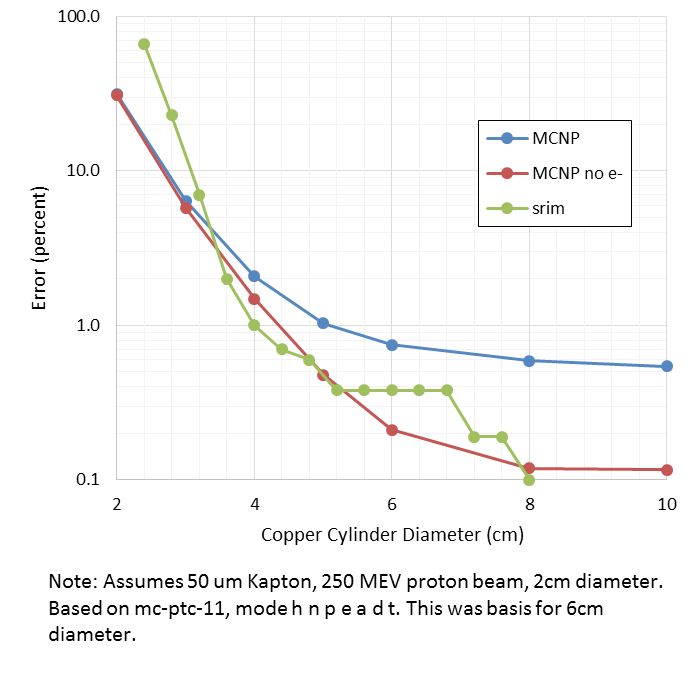
\includegraphics[width=4in]{fig_error_diameter.png}
  \caption{Signal Error vs Diameter and Simulation Method}
  \label{fig:error_diameter}
\end{figure}

The same calculation was repeated with proton tallies alone, i.e., without any secondary electrons. This shows that if electrons had been completely ignored, the MCNP6 results would have been similar to the SRIM model and a diameter of 8 cm would have seemed reasonable.

The distribution of proton collisions from 50 beam protons is in Fig.~\ref{fig:mcnp_tracks}. The distribution of 6 other particles (born of 50 Protons) is in Fig.~\ref{fig:mcnp_dist}; neutrons go everywhere. The distribution of electrons (just type SE$_{!h}$) is similar to photons. Table \ref{tab:mcnp_neutral_crossing} shows the boundary crossings of neutral particles. In the problem there are about two neutral particle boundary crossings per beam proton.

Table \ref{tab:mcnp_charge_crossing} shows the breakdown of gain from various charged particles for given directions and copper surfaces. This assumes 250 MeV Proton Beam, 6cm Copper Diameter and 50 microns kapton. The effect of secondary electrons produced directly by proton collisions (SD$_h$) is not included.

\begin{figure}[H]
  \centering
  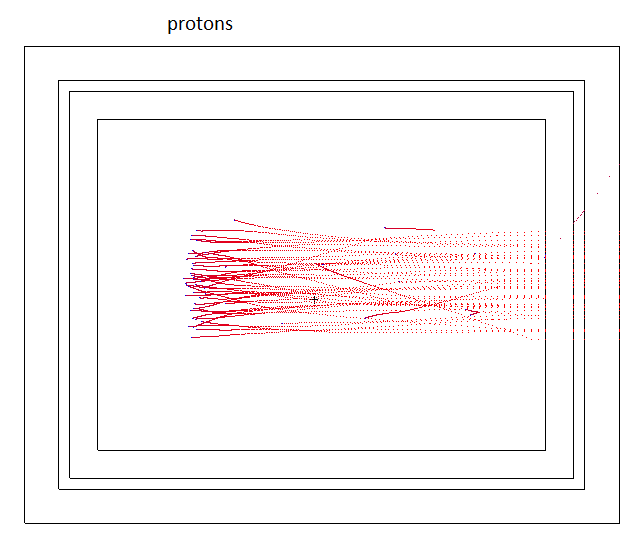
\includegraphics[width=4in]{fig_mcnp_tracks.png}
  \caption{Distribution of 50 Protons of Energy 250 MeV using MCNP6. Note the singular backscatter.}
  \label{fig:mcnp_tracks}
\end{figure}

\begin{figure}[H]
        \centering
        \begin{subfigure}[b]{0.2\textwidth}
                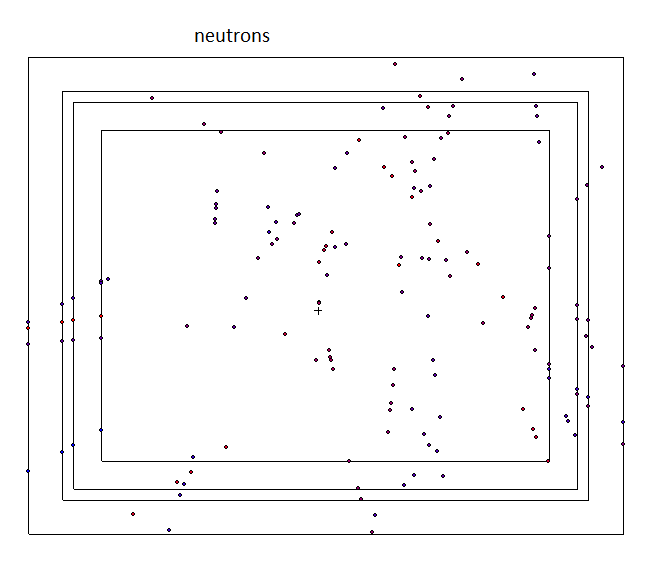
\includegraphics[width=\textwidth]{fig_mcnp_dist_n.png}
                \label{fig:mcnp_dist_n}
        \end{subfigure}
        %
        \begin{subfigure}[b]{0.2\textwidth}
                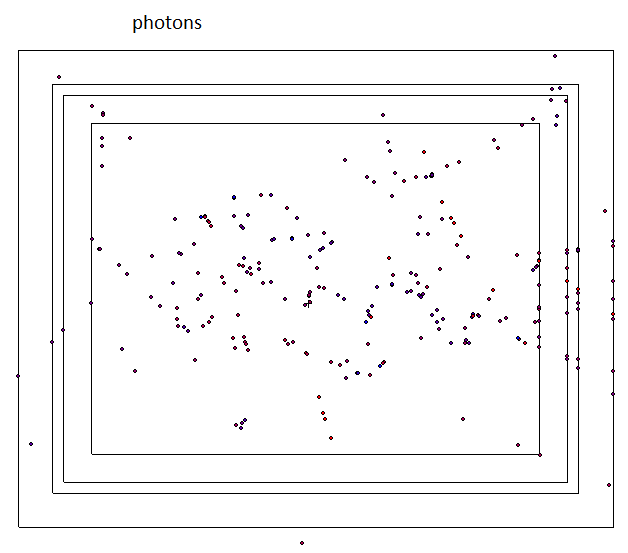
\includegraphics[width=\textwidth]{fig_mcnp_dist_ph.png}
                \label{fig:mcnp_dist_ph}
        \end{subfigure}
        %
        \begin{subfigure}[b]{0.2\textwidth}
                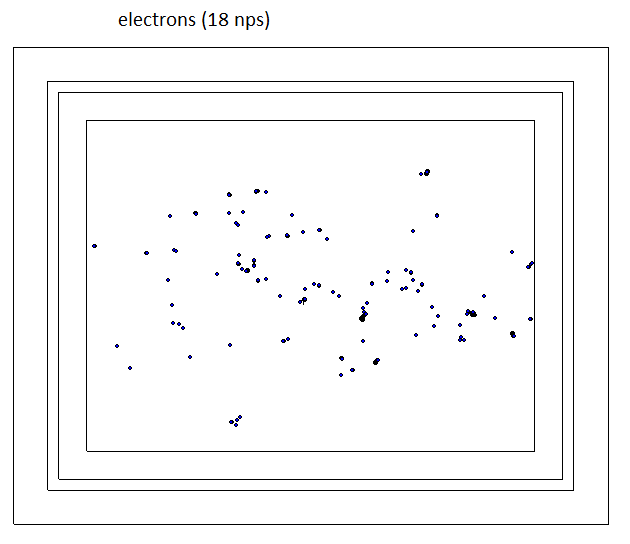
\includegraphics[width=\textwidth]{fig_mcnp_dist_e.png}
                \label{fig:mcnp_dist_e}
        \end{subfigure}
        
        \begin{subfigure}[b]{0.2\textwidth}
                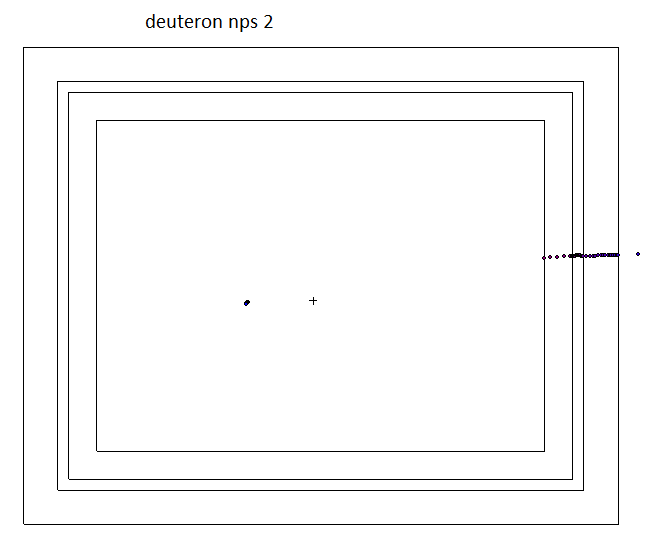
\includegraphics[width=\textwidth]{fig_mcnp_dist_d.png}
                \label{fig:mcnp_dist_d}
        \end{subfigure}
        %
        \begin{subfigure}[b]{0.2\textwidth}
                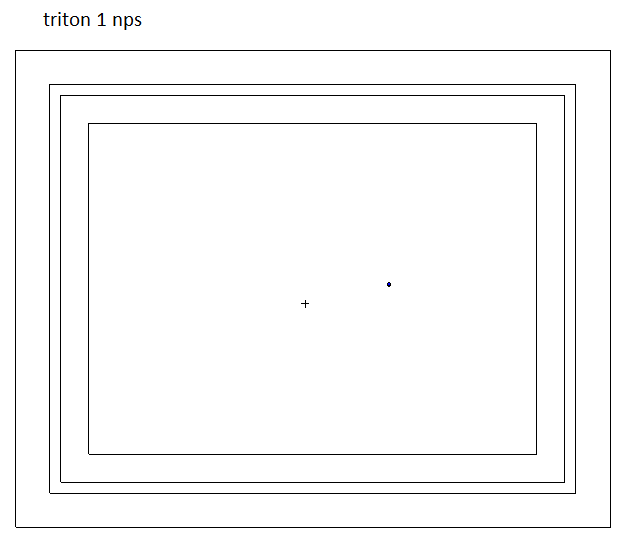
\includegraphics[width=\textwidth]{fig_mcnp_dist_t.png}
                \label{fig:mcnp_dist_t}
        \end{subfigure}
        %
        \begin{subfigure}[b]{0.2\textwidth}
                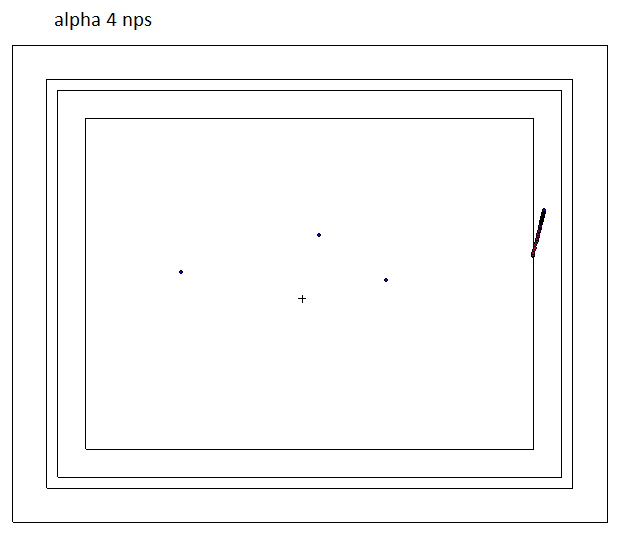
\includegraphics[width=\textwidth]{fig_mcnp_dist_a.png}
                \label{fig:mcnp_dist_a}
        \end{subfigure}
        \caption{Distribution of six other particles}
        \label{fig:mcnp_dist}
\end{figure}

It is worth examining the behavior of the model. Kapton thickness (25, 50 and 75 microns) seems to make no difference in gain. Neither do the inclusion of tallies for deuterons, tritons and alphas, although the MCNP output file notes the absence of production cross-sections for these particles\footnote{The absence of ion production XS noted in the MCNP output file vs the presence of ions in the run needs to be checked out.}. All of the figures and tables below were for the case of 6cm diameter, 50 microns of kapton and 50 beam protons of energy 250 MeV.

\begin{table}
  \centering
  \caption{Charges Crossing Copper Surfaces (fraction per proton source) assuming 250 MeV Proton Beam, 6 cm Copper diameter, 50 microns of Kapton, and no SE$_\text{h}$}
  \begin{tabular}{clcccc}
    \toprule
    Particle & tally & face & cylinder & end & total \\
    \midrule
    n  & in & \num{0.00065} & \num{0.00044} & \num{0.10692} & \num{0.10801} \\
       & out & \num{0.14874} & \num{0.67867} & \num{0.00007} & \num{0.82747} \\
    \midrule
    $\gamma$ & in & \num{0.00038} & \num{0.00070} & \num{0.00011} & \num{0.00119} \\
             & out & \num{0.17603} & \num{0.65051} & \num{0.07812} & \num{0.90466} \\
    \bottomrule
  \end{tabular}
  \label{tab:mcnp_neutral_crossing}
\end{table}

\begin{table}
  \centering
  \caption{Charges Crossing Copper Surfaces (fraction per proton source) assuming 250 MeV Proton Beam, 6 cm Copper diameter, 50 microns of Kapton, and no SE$_\text{h}$}
  \begin{tabular}{clcccc}
    \toprule
    Particle & tally & face & cylinder & end & total \\
    \midrule
       & in & \num{0.99997} & \num{0.00000} & \num{0.00000} & \num{0.99997} \\
    P+ & out & \num{0.00055} & \num{0.00123} & \num{0.00023} & \num{0.00201} \\
       & total & \num{0.99941} & \num{0.00123} & \num{0.00023} & \num{0.99796} \\
    \midrule
       & in & \num{0.00031} & \num{0.00087} & \num{0.00010} & \num{0.00128} \\
    E\ (no SE$_\text{h}$) & out & \num{0.00149} & \num{0.00450} & \num{0.00051} & \num{0.00650} \\
       & total & \num{0.00119} & \num{0.00362} & \num{0.00042} & \num{0.00523} \\
    \midrule
       & in & \num{0.00003} & \num{0.00000} & \num{0.00000} & \num{0.00003} \\
     d & out & \num{0.00007} & \num{0.00006} & \num{0.00002} & \num{0.00015} \\
       & total & \num{0.00004} & \num{0.00006} & \num{0.00002} & \num{0.00012} \\
    \midrule
       & in & \num{0.00002} & \num{0.00000} & \num{0.00000} & \num{0.00002} \\
     t & out & \num{0.00003} & \num{0.00006} & \num{0.00002} & \num{0.00003} \\
       & total & \num{0.00001} & \num{0.00006} & \num{0.00002} & \num{0.00001} \\
    \midrule
       & in & \num{0.00003} & \num{0.00000} & \num{0.00000} & \num{0.00003} \\
     a & out & \num{0.00003} & \num{0.00000} & \num{0.00000} & \num{0.00003} \\
       & total & \num{0.00000} & \num{0.00000} & \num{0.00000} & \num{0.00000} \\
    \midrule
       & in & \num{0.99974} & \num{0.00087} & \num{0.00010} & \num{1.00124} \\
    Signal & out & \num{0.00082} & \num{0.00320} & \num{0.00026} & \num{0.00851} \\
       & total & \num{0.99823} & \num{0.00485} & \num{0.00065} & \num{0.99273} \\
    \bottomrule
  \end{tabular}
  \label{tab:mcnp_charge_crossing}
\end{table}

\subsection{Geant4 Simulation}

The units of signal gain are $\frac{Q_{net}}{Q_P}$, where $Q_{net}$ is the net transfer of charge into the cup, and $Q_P$ is the net charge of the million protons irradiating the cup.  Charges entering and leaving the primary Kapton film covering the copper are subject to the linear proportion behavior defined in Eq.~\ref{eqn:s_KA}.  Table \ref{tab:geant4_data} shows a sample output of each model in both air and vaccuum, the latter to remove oversaturation of beta emissions from the air due to delta-ray production (LATER: citation needed).

\begin{table}[H]
  \centering
  \caption{Predicted Gain from High-Energy Protons using Geant4}
  \begin{tabular}{lccccc}
    \toprule
    Model & Energy (MeV) & (-Ag/KA) & (-Ag/KA) \emph{in vacuo} & (+Ag/KA) & (+Ag/KA) \emph{in vacuo} \\
    \midrule
    S59 & 70.03  & \num{0.953588} & \num{1.00036} & \num{0.983320} & \num{0.979287} \\
        & 100.46 & \num{0.967417} & \num{1.00068} & \num{0.982263} & \num{0.979775} \\
        & 130.52 & \num{0.975593} & \num{1.00118} & \num{0.982531} & \num{0.981160} \\
        & 160.09 & \num{0.981094} & \num{1.00177} & \num{0.983127} & \num{0.982672} \\
        & 190.48 & \num{0.985111} & \num{1.00238} & \num{0.984641} & \num{0.983603} \\
        & 221.06 & \num{0.988151} & \num{1.00314} & \num{0.986131} & \num{0.985152} \\
        & 250.00 & \num{0.990298} & \num{1.00358} & \num{0.987536} & \num{0.986296} \\
    \midrule
    S100 & 70.03 & \num{0.953827} & \num{1.00036} & \num{0.983731} & \num{0.979531} \\
        & 100.46 & \num{0.966795} & \num{1.00072} & \num{0.982408} & \num{0.979939} \\
        & 130.52 & \num{0.975725} & \num{1.00121} & \num{0.982508} & \num{0.980993} \\
        & 160.09 & \num{0.981055} & \num{1.00180} & \num{0.983059} & \num{0.982456} \\
        & 190.48 & \num{0.985189} & \num{1.00245} & \num{0.984910} & \num{0.983649} \\
        & 221.06 & \num{0.988149} & \num{1.00326} & \num{0.986215} & \num{0.985251} \\
        & 250.00 & \num{0.990324} & \num{1.00349} & \num{0.987278} & \num{0.986103} \\
    \midrule
    S200 & 70.03 & \num{0.954372} & \num{1.00037} & \num{0.983544} & \num{0.979594} \\
        & 100.46 & \num{0.966915} & \num{1.00068} & \num{0.982554} & \num{0.979769} \\
        & 130.52 & \num{0.975377} & \num{1.00126} & \num{0.982246} & \num{0.981054} \\
        & 160.09 & \num{0.980998} & \num{1.00178} & \num{0.983405} & \num{0.982137} \\
        & 190.48 & \num{0.985217} & \num{1.00244} & \num{0.984706} & \num{0.983760} \\
        & 221.06 & \num{0.988312} & \num{1.00320} & \num{0.986402} & \num{0.984905} \\
        & 250.00 & \num{0.990213} & \num{1.00343} & \num{0.987178} & \num{0.985874} \\
    \bottomrule
  \end{tabular}
  \label{tab:geant4_data}
\end{table}

Fig.~\ref{fig:G4_dist} depicts the tracks of particles given the simulation of 50 250 MeV protons entering the S59 model.  The track color corresponds to particle charge, red for negative, blue for positive, and green neutral.  As observed in the MCNP6 simulation, neutrons are scattered everywhere; for the most part, electrons created in the Faraday Cup do not travel far, as expected given their low-energy production and high stopping-power in copper.

\begin{figure}[H]
  \centering
  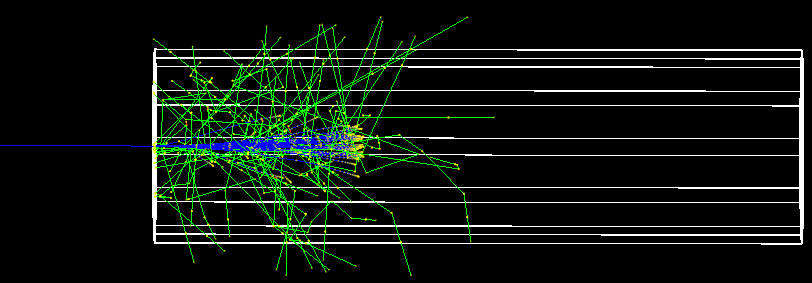
\includegraphics[width=5in]{fig_G4_dist.png}
  \caption{Distribution of 50 Protons of Energy 250 MeV using Geant4.}
  \label{fig:G4_dist}
\end{figure}


%%%%%%%%%%%%%%%%%%%%%%%%%%%%%%%%%%%%%%%%%%%%%%%%%%%%%%%%%%%%%%%%%%%%%
\section{Discussion}

It is known that MCNP does not track electrons secondary to protons. Therefore, there are delta rays and secondary electrons from protons that have not been accounted for. This means that the error is greater than has been portrayed. This needs further investigation because it is shown in Fig.~\ref{fig:error_diameter} that electrons (just the SE$_{!h}$) have an impact on the choice of diameter.

The electrons that are included are those that are secondary to the particle cascade subsequent to protons. For example, there are electrons secondary to photons that come from neutrons that come from protons. Table \ref{tab:mcnp_neutral_crossing} shows that there are almost 2 neutral particles crossing the Faraday Cup boundary per beam proton.

It is important to note that the addition of deuterons, tritons and alphas changes the gain by -0.0002\footnote{See mc-ptc-11-3.0-f for effect of deuterons, tritons, and alphas.}, and that there were no proton creation cross-sections for Ag-107, so it was substituted for Ag-109 which makes up about 2/3 of the silver.

In pursuit of the optimization of this portable Faraday Cup, we considered many variants of applicable theoretical models to corroborate with available experimental data.  Fig. \ref{fig:comp_results} depicts a very convincing similarity in behavior between the HIT beam stop measurements, and the simulation of the copper Faraday Cup in air without the \emph{no} silver/Kapton layer.

\begin{figure}[h]
  \centering
  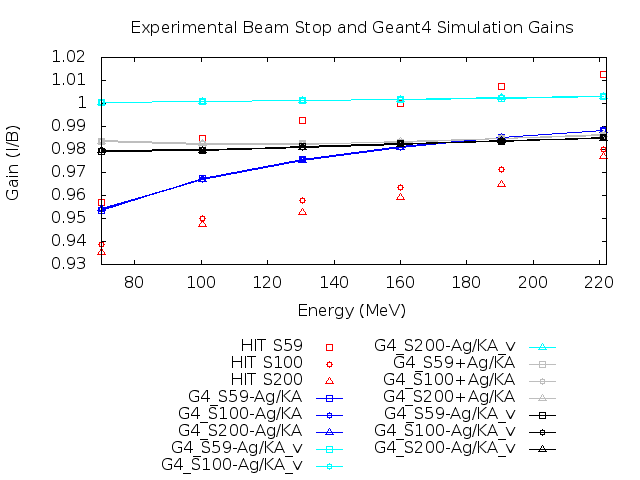
\includegraphics[width=5in]{fig_results.png}
  \caption{Comparison of Geant4 output and HIT measurement.  Generated with Gnuplot.}
  \label{fig:comp_results}
\end{figure}


%%%%%%%%%%%%%%%%%%%%%%%%%%%%%%%%%%%%%%%%%%%%%%%%%%%%%%%%%%%%%%%%%%%%%
\section{Conclusions}


%%%%%%%%%%%%%%%%%%%%%%%%%%%%%%%%%%%%%%%%%%%%%%%%%%%%%%%%%%%%%%%%%%%%%
\section{Acknowledgments}

We would like to express our sincerest gratitude to Paul Romano and Tom Sutton, who provided the template for this paper.

%%%%%%%%%%%%%%%%%%%%%%%%%%%%%%%%%%%%%%%%%%%%%%%%%%%%%%%%%%%%%%%%%%%%%
\setlength{\baselineskip}{12pt}

\bibliographystyle{mc2015}
\bibliography{references}

%%%%%%%%%%%%%%%%%%%%%%%%%%%%%%%%%%%%%%%%%%%%%%%%%%%%%%%%%%%%%%%%%%%%%
\appendix
\section{mc-ptc-11-3.0-f?}

Code bits?

\pageref{lastpage}
\end{document}
